\documentclass[fullscreen=true, bookmarks=true, hyperref={pdfencoding=unicode}]{beamer}
\usepackage[utf8]{inputenc}                                % Кодировка
\usepackage[english,russian]{babel}                        % Переносы
\usepackage{xcolor}                                        % Работа с цветом
\usepackage{amsmath,amssymb,amsfonts}                      % Символы АМО
\usepackage{graphicx}                                      % Графика
\usepackage[labelsep=period]{caption}                      % Разделитель в подписях к рисункам и таблицам
\usepackage{hhline}                                        % Для верстки линий в таблицах
\usepackage{tikz}                                          % Для простых рисунков в документе
\usepackage{fancybox}                                      % Пакет для отрисовки рамок
\usepackage{verbatim}                                      % Для вставки кода в презентацию
\usepackage{animate}                                       % Для вставки видео в презентацию
\usepackage{xmpmulti}                                      % Для вставки gif в презентацию
\usepackage{multirow}
\usepackage{mathrsfs}
\usepackage[normalem]{ulem}

\usetikzlibrary{arrows, snakes, backgrounds}                 % Для отрисовки стрелок
\usetikzlibrary{positioning, fit, arrows.meta, shapes, calc}
% used to avoid putting the same thing several times...
% Command \empt{var1}{var2}
\newcommand{\empt}[2]{$#1^{\langle #2 \rangle}$}

\graphicspath{{images/}}                                   % Путь до рисунков
\setbeamertemplate{caption}[numbered]                      % Включение нумерации рисунков

\definecolor{links}{HTML}{2A1B81}                          % blue for url links
\hypersetup{colorlinks,linkcolor=,urlcolor=links}          % nothing for others

\usetheme{boxes}
\usecolortheme{crane}

\usepackage{pythonhighlight}

\newtheorem*{question}{Вопрос}

\title{Лекция 11. Многорукие бандиты}
\author{Александр Юрьевич Авдюшенко}
\institute{МКН СПбГУ}
\date{28 апреля 2022}
\titlegraphic{
\includegraphics[keepaspectratio,width=0.5\textwidth]{logo_fmkn.png}}


\begin{document}
%\unitlength=2mm

% выводим заглавие
\begin{frame}
\transdissolve[duration=0.2]
\titlepage
\end{frame}


\begin{frame}
  \frametitle{Пятиминутка}
  \begin{itemize}
    \item Назовите три основных подхода к построению моделей ранжирования
    \item Расшифруйте аббревиатуру RMSE
    \item Перечислите нетривиальные свойства, влияющие на качество рекомендаций, которые трудно измерять
  \end{itemize}
\end{frame}


\begin{frame}
  \frametitle{Постановка задачи}

  \begin{itemize}
    \item До этого момента мы либо восстанавливали функцию по обучающей выборке $(X, Y)$ (supervised learning), либо искали структуру в наборе объектов $X$ (unsupervised learning)
    \item Как происходит обучение в реальной жизни? Обычно делаем какое-то действие и получаем результат, постепенно обучаясь
  \end{itemize}
\end{frame}


\begin{frame}
  \frametitle{Ещё мотивация}
  \framesubtitle{Например, нам нужно выбрать главную страницу сайта магазина открыток, чтобы привлечь пользователя}

  \begin{columns}
      \begin{column}{.5\paperwidth}
        \begin{center}
          
\includegraphics[keepaspectratio,
                           height=.5\paperheight]{hi-1.jpg}
        \end{center}
      \end{column}
      \begin{column}{.5\paperwidth}
        \begin{center}
          
\includegraphics[keepaspectratio,
                           height=.5\paperwidth]{hi-2.jpg}
        \end{center}
      \end{column}
  \end{columns}

\end{frame}


\begin{frame}
  \frametitle{Какие подходы есть?}

  \begin{itemize}
    \item A/B тестирование — потенциально плохие варианты видят многие пользователи
    \item многорукие бандиты — частный случай обучения с подкреплением
  \end{itemize}
\end{frame}


\begin{frame}
  \frametitle{Однорукий бандит Бернулли}

  \begin{center}
    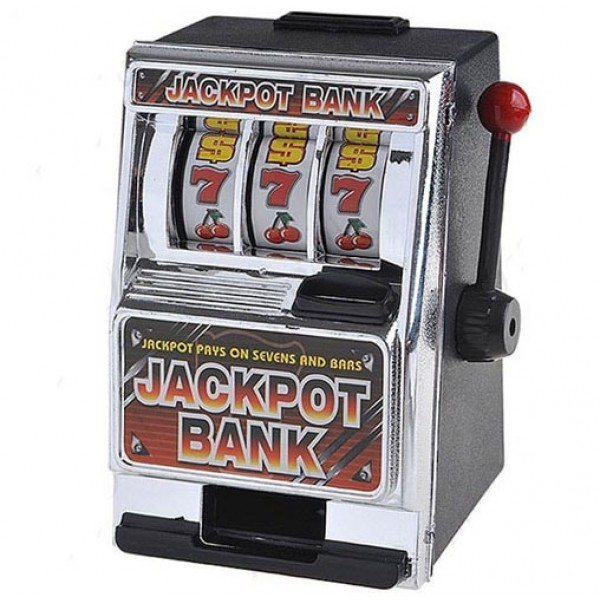
\includegraphics[keepaspectratio,
                     width=.5\paperwidth]{data-kopilkabandit.jpg}
  \end{center}

  Вероятность выиграть $\theta = 0.05$
\end{frame}


\begin{frame}
  \frametitle{Многорукие бандиты}

  \begin{columns}
      \begin{column}{.25\paperwidth}
        \begin{center}
          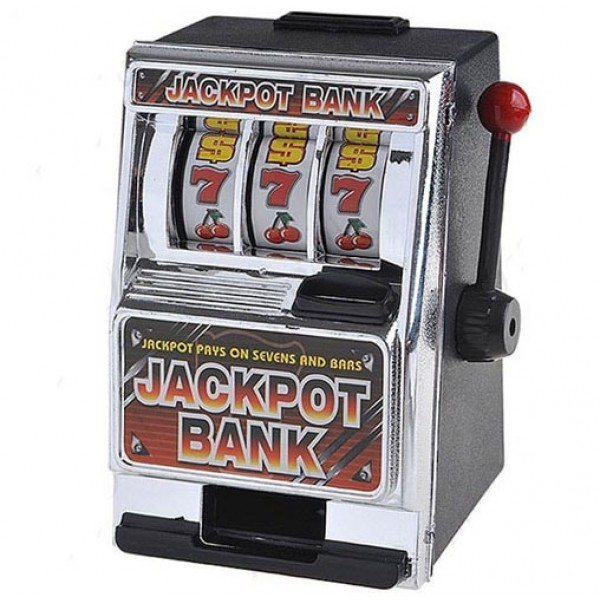
\includegraphics[keepaspectratio,
                           width=.2\paperwidth]{data-kopilkabandit.jpg}

        Вероятность выиграть $\theta = 0.02$
        \end{center}
      \end{column}
      \begin{column}{.25\paperwidth}
        \begin{center}
          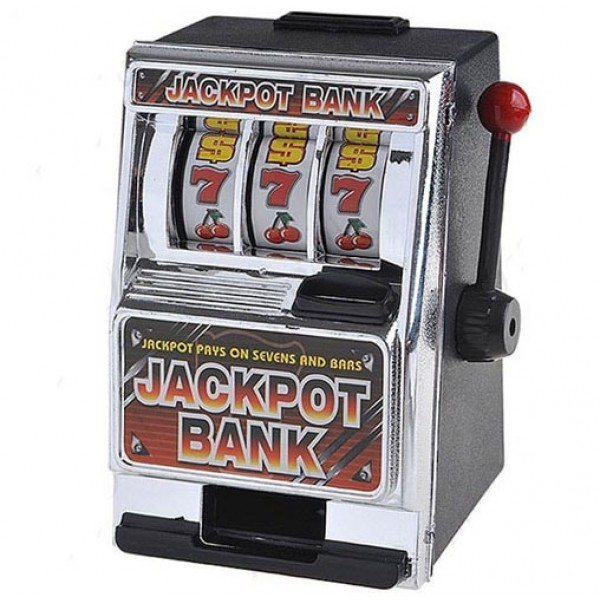
\includegraphics[keepaspectratio,
                           width=.2\paperwidth]{data-kopilkabandit.jpg}

          Вероятность выиграть $\theta = 0.01 (\min)$
        \end{center}
      \end{column}
      \begin{column}{.25\paperwidth}
        \begin{center}
          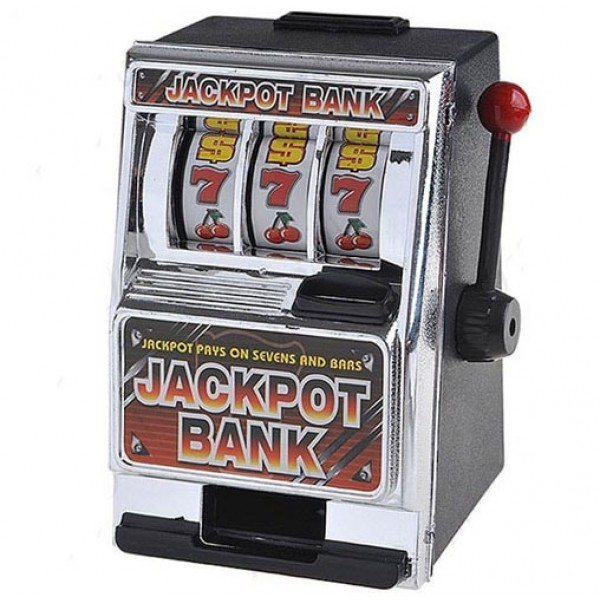
\includegraphics[keepaspectratio,
                           width=.2\paperwidth]{data-kopilkabandit.jpg}

        Вероятность выиграть $\theta = 0.05$
        \end{center}
      \end{column}
      \begin{column}{.25\paperwidth}
        \begin{center}
          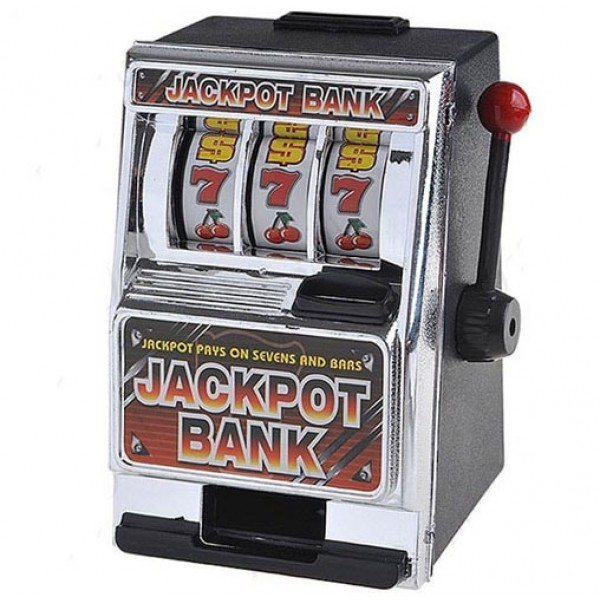
\includegraphics[keepaspectratio,
                           width=.2\paperwidth]{data-kopilkabandit.jpg}

           Вероятность выиграть $\theta = 0.1 (\max)$
        \end{center}
      \end{column}
  \end{columns}

  \vspace{1cm}
  Мы не знаем истинные вероятности, но хотим придумать стратегию, максимизирующую выигрыш (награду).
\end{frame}


\begin{frame}
  \frametitle{Математическая постановка задачи}

  Даны возможные действия $$x_1, \dots, x_n$$

  На очередной итерации $t$ при каждом совершаемом действии $x^t_i$ мы получаем ответ $$ y^t_i \sim q(y|x^t_i, \Theta),$$

  который приносит нам награду {\bf reward} $$r_i^t = r(y^t_i)$$

  Существует оптимальное действие $x_{i^*}$ (иногда $x_{i^*_t}$) $$\forall i:\ E(r_{i^*_t}^t) \geq E(r^t_i)$$
\end{frame}


\begin{frame}
  \frametitle{Мера качества}

  \begin{question}
    Как оценивать различные стратегии?
  \end{question}

  \pause
  Мерой качества алгоритма многоруких бандитов $a$ обычно является {\bf regret} $$ R(a) = \sum\limits_{t=1}^T \left(E(r_{i^*_t}^t) - E(r_{i^a_t}^t) \right)$$

  \vspace{1cm}
  В синтетических условиях (когда знаем вероятности) можно рассмотреть $$ E\left( R \right) = \int\limits_{\Theta} R(a)d\Theta$$
\end{frame}


\begin{frame}
  \frametitle{$\varepsilon$-жадный подход}

  \begin{center}
    
\includegraphics[keepaspectratio,
                     width=.8\paperwidth]{greedy_billy.jpg}
  \end{center}
\end{frame}


\begin{frame}
  \frametitle{Жадный подход}

  \begin{itemize}
    \item на основе исторических данных оценить распределение параметров модели $P(\Theta|X)$
    \item всегда использовать действие, ведущее к наибольшему выигрышу в среднем на основании полученного распределения
  \end{itemize}

   $$ x_k = \arg\max\limits_{x_k} E_{y|x_k, \hat \Theta}\left( r(y)\right),$$

  где $\hat \Theta = E \Theta$
\end{frame}


\begin{frame}
  \frametitle{Формула Байеса}
  \framesubtitle{напоминание}

  $$ P(\Theta|Y) = \frac{Q(Y|\Theta)P(\Theta)}{Q(Y)}$$

  \pause
  $$ P_t(\Theta|Y_t) = \frac{q(y^t|x^t, \Theta) P_{t-1}(\Theta|Y_{t-1})}{q(y^t|x^t)}$$

  \pause
  \begin{question}
    Что получится для бандита Бернулли?
  \end{question}
\end{frame}


\begin{frame}
  \frametitle{Пример. Применение формулы Байеса для бандита Бернулли}

  $Q(Y|\Theta)$ представляется в виде $Q(Y|\theta_1), Q(Y|\theta_2),\dots,Q(Y|\theta_k)$, где

  $$ Q(Y|\theta) = C_{T_i}^{\sum\limits_{t \in |T_i|} r_i^t}
  \theta^{\sum\limits_{t \in |T_i|} r_i^t} (1-\theta)^{|T_i| - \sum\limits_{t \in |T_i|}r_i^t}
  $$

  $ \Theta = \{\theta_1, \theta_2, \dots, \theta_K\} $, $\theta_k$ — коэффициент для $k$-го бандита (параметр распределения Бернулли)

  $$y_k \sim \text{Bernoulli}(\theta_k)$$

\end{frame}


\begin{frame}
  Распределение параметров распределений Бернулли — Бета-распределение:

  $$ p(\theta_k) = \frac{\Gamma(\alpha_k + \beta_k)}{\Gamma(\alpha_k)\Gamma(\beta_k)}
     \theta_k^{\alpha_k - 1} (1-\theta_k)^{\beta_k - 1}$$

     \begin{center}
       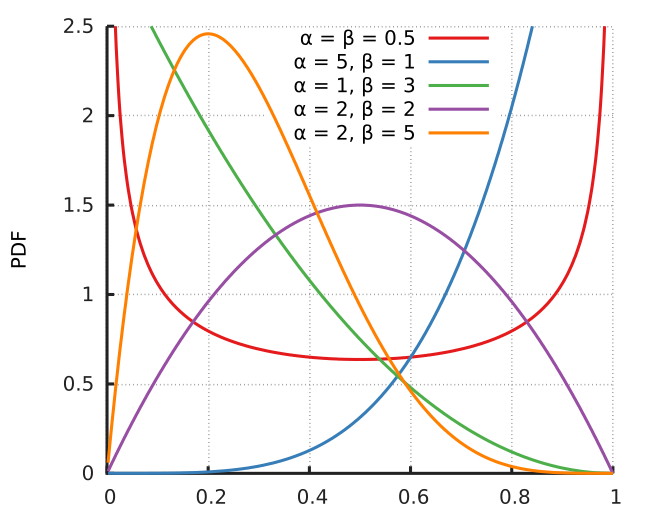
\includegraphics[keepaspectratio,
                        width=.5\paperwidth]{650px-Beta_distribution_pdf.png}
     \end{center}

  Схема обновления распределения параметров после $t$-го шага:

  $$ (\alpha_k, \beta_k) \leftarrow (\alpha_k, \beta_k) + (r^t_k,1 - r^t_k) $$

  $r^t_k$ — награда в случае, если на шаге $t$ мы выбрали действие $k$

  $r^t_k = r(y^t_k) = y^t_k$
\end{frame}


\begin{frame}
   \frametitle{Проблемы с жадностью}

   \begin{center}
     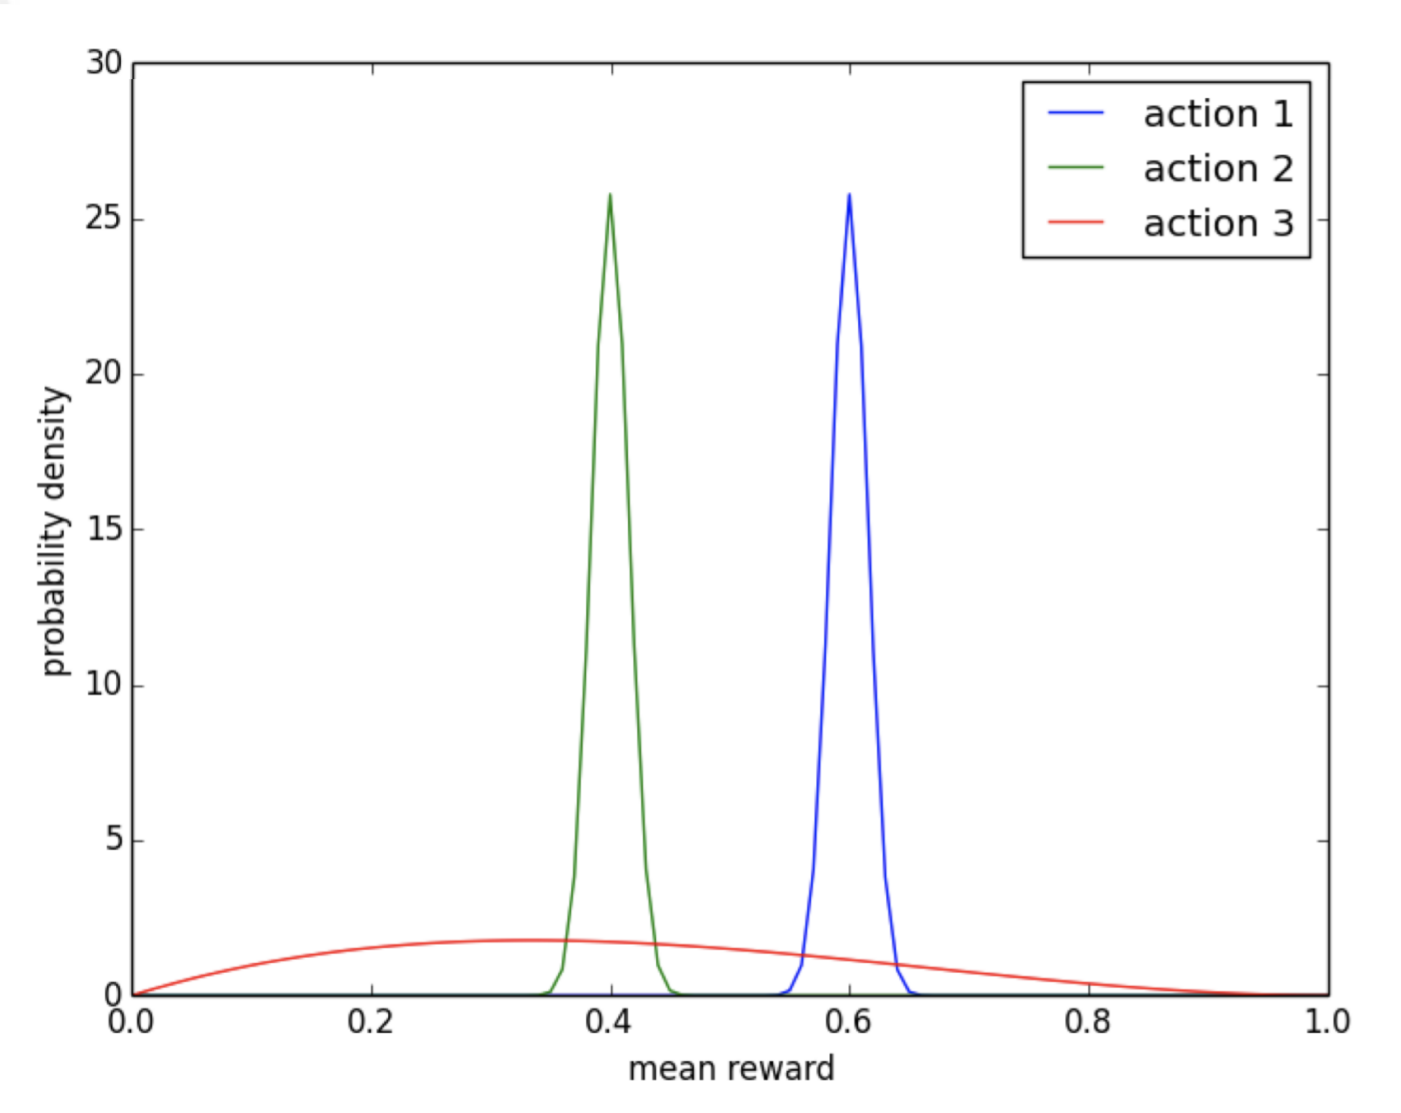
\includegraphics[keepaspectratio,
                      width=.5\paperwidth]{greedy_example.png}
   \end{center}

   Апостериорные распределения после того, как:

   \begin{itemize}
     \item бандит 1 был использован 1000 раз и дал выигрыш 600 раз
     \item бандит 2 был использован 1000 раз и дал выигрыш 400 раз
     \item бандит 3 был использован 3 раза и дал выигрыш 1 раз
   \end{itemize}
\end{frame}


\begin{frame}
  \frametitle{$\varepsilon$-жадный алгоритм}

  \begin{itemize}
    \item на основе исторических данных оценить распределение параметров модели $\Theta$, $P(\Theta|X)$
    \item с вероятностью $\varepsilon$ выбирать случайное действие
    \item с вероятностью $1-\varepsilon$ выбирать действие, ведущее к наибольшему выигрышу в среднем на основании полученного распределения $$ x_k = \arg\max_{x_k} E_{y|x_k, \hat \Theta} [r(y)],$$
    где $\hat \Theta = E \Theta$
   \item повторить
  \end{itemize}

  Недостатки
  \begin{itemize}
    \item[-] изучение новых возможностей полностью случайно и никак не зависит от уже известной информации
    \item[-] непонятно, когда нужно прекращать исследовать и начинать использовать
  \end{itemize}
\end{frame}


\begin{frame}
  \frametitle{Сэмплирование Томпсона}

  \begin{itemize}
    \item на основе исторических данных оценить распределение параметров модели $\Theta$, $P(\Theta|X)$
    \item семплировать один раз $\hat \Theta$ из его текущего распределения $P(\Theta|X)$
    \item выбирать действие, ведущее к наибольшему выигрышу в среднем на основании полученного распределения $$ x_k = \arg\max_{x_k} E_{y|x_k, \hat \Theta} [r(y)]$$
    \item повторить
  \end{itemize}

  \vspace{1cm}

  \noindent\rule{8cm}{0.4pt}

  {\small
  {\it Daniel J. Russo, Benjamin Van Roy, Abbas Kazerouni, Ian Osband and Zheng Wen} \href{https://arxiv.org/pdf/1707.02038.pdf}{«A Tutorial on Thompson Sampling», 2018}}

\end{frame}


\begin{frame}
  \frametitle{Сэмплирование Томпсона. Пример}

  \begin{center}
    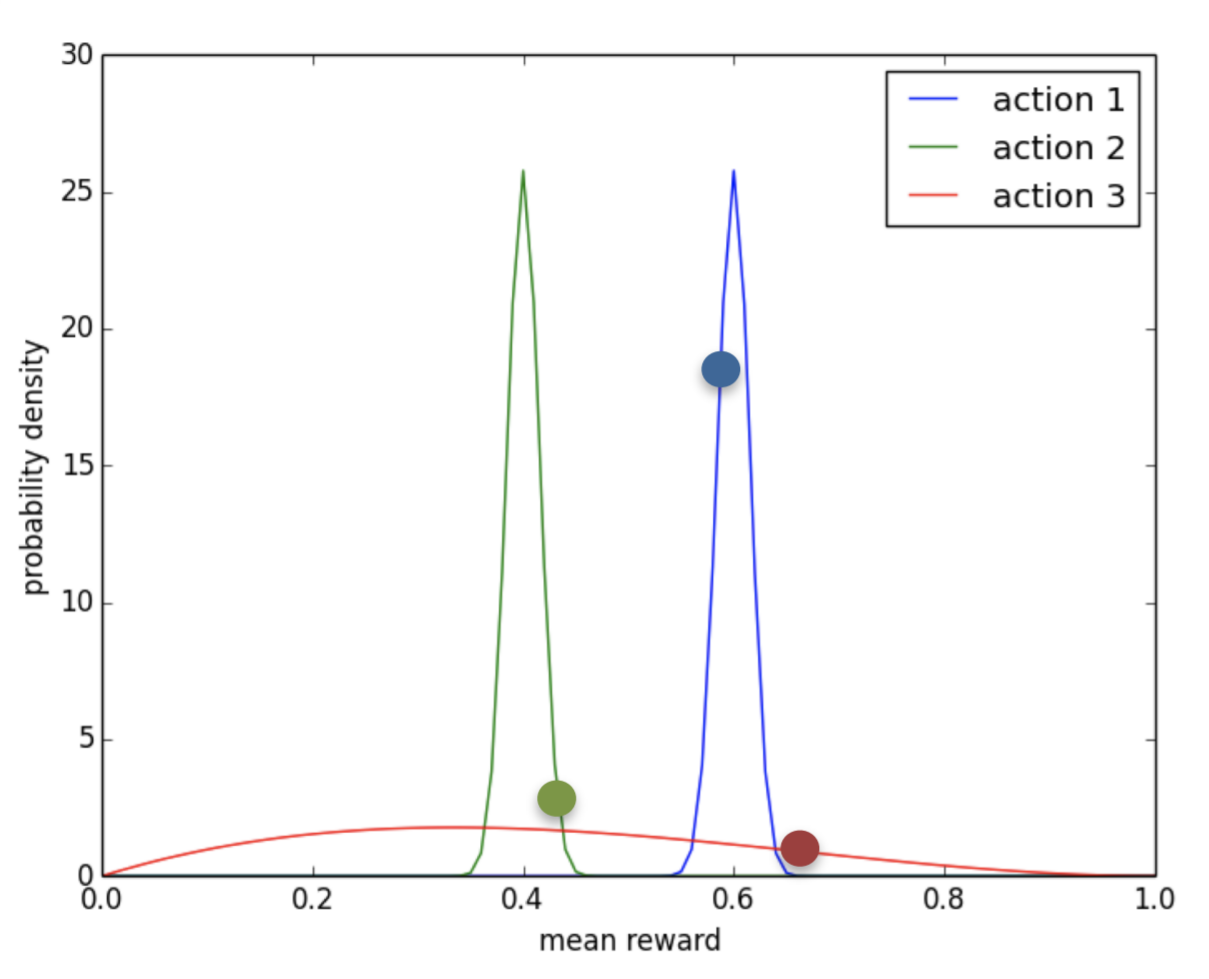
\includegraphics[keepaspectratio,
                     width=.5\paperwidth]{thompson_example.png}
  \end{center}

  Сэмплировали, например:
  \begin{itemize}
    \item $\theta_1$ = 0.59
    \item $\theta_2$ = 0.45
    \item $\theta_3$ = 0.67
  \end{itemize}

  Выбираем action3
\end{frame}


\begin{frame}
  \frametitle{Сходимость к оптимальным значениям}

  $\theta_1 = 0.9, \theta_2 = 0.8, \theta_3 = 0.7$, априорное распределение равномерное. Проводим 1000 независимых испытаний по 1000 шагов $t$ в каждом.
  \begin{center}
    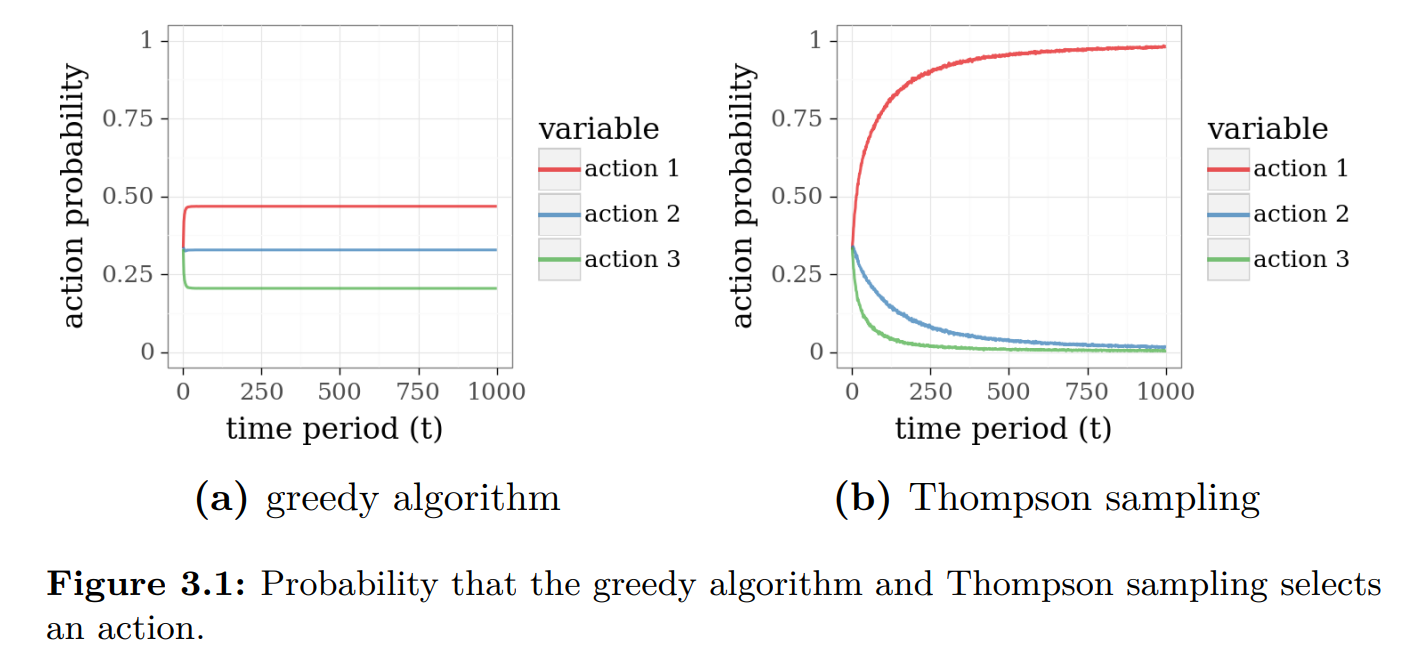
\includegraphics[keepaspectratio,
                     width=.9\paperwidth]{greedy_tompson.png}

     {\small В каждой точке — доля испытаний, в которой выбрано соотвествующее действие}
  \end{center}

\end{frame}


\begin{frame}
  \frametitle{Теоретические оценки}

  {\bf Сверху}

  $$ \max\limits_{\theta^\prime} \mathbb{E}[\text{Regret}(T) | \theta = \theta^\prime] = O\left(\sqrt{KT \log(T)} \right)$$

  {\bf Снизу}
  Показано, что существует распределение такое, что $$ \max\limits_{\theta^\prime} \mathbb{E}[\text{Regret}(T) | \theta = \theta^\prime] = \Omega\left(\sqrt{KT } \right)$$

\end{frame}


\begin{frame}
  \frametitle{Пример. Путь в графе}

  $G(V, E)$

  $x_t = e_{1^\prime} \to e_{2^\prime} \dots \to e_{U^\prime}$

  $r_t = - \sum\limits_{e \in x_t} y_e^t$

  \begin{center}
    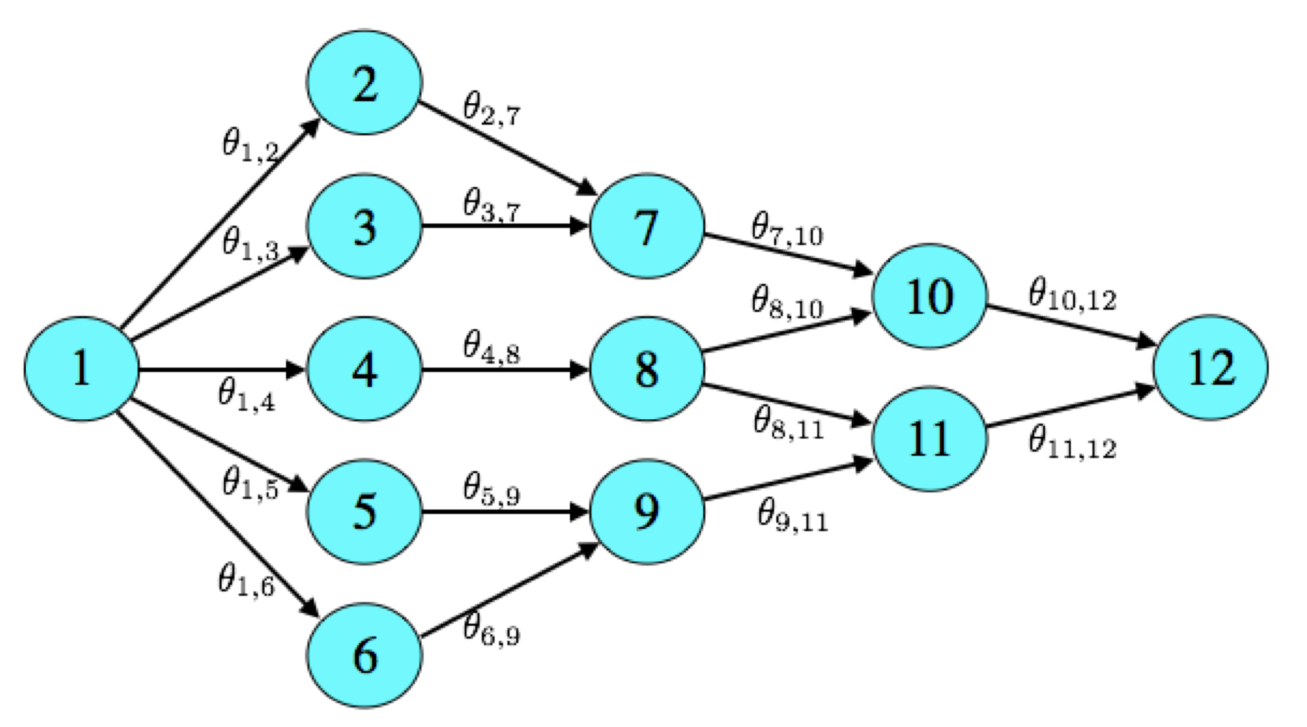
\includegraphics[keepaspectratio,
                     width=.7\paperwidth]{graph_path.png}
  \end{center}
\end{frame}


\begin{frame}
  \frametitle{Пример. Путь в графе}

  $ \theta_e \sim LN(\mu_e, \sigma_e^2)$ (логнормальное распределение)

  Математическое ожидание $E[\theta_e] = e^{\mu_e + \sigma_e^2/2}$


  \begin{center}
    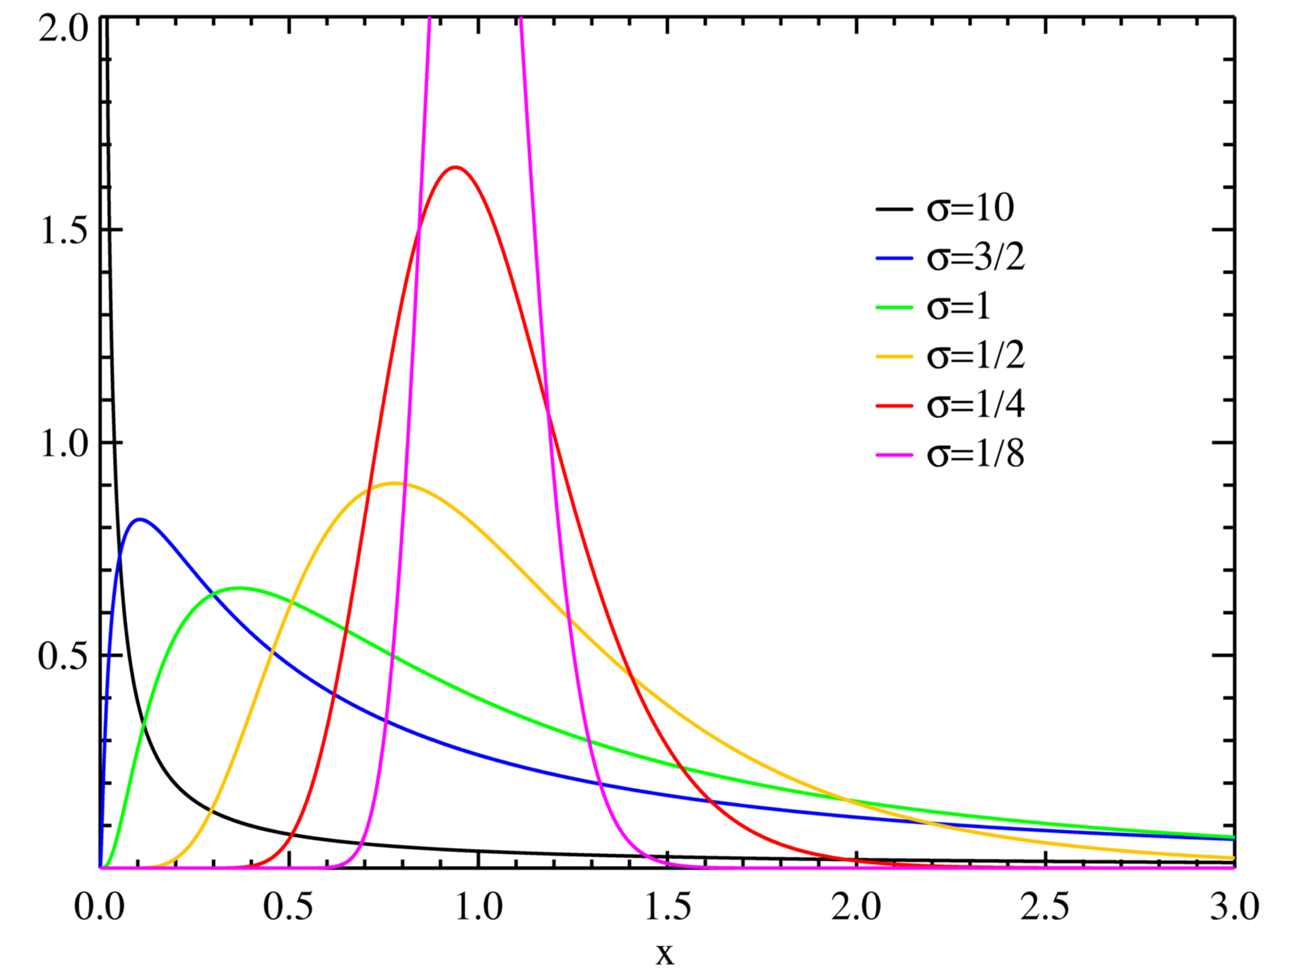
\includegraphics[keepaspectratio,
                     width=.6\paperwidth]{Lognormal_distribution_PDF.png}

    Плотность вероятности, $\mu = 0$
  \end{center}

  $y_e^t \sim LN(\ln(\theta_e) - s^2/2, s^2)$,
  $E[y^t_e|\theta_e] = \theta_e$

\end{frame}


\begin{frame}
  Обновление распределений параметров

  $$ (\mu_e, \sigma_e^2) \leftarrow
  \left(
  \frac{\frac{1}{\sigma_e^2}\mu_e + \frac{1}{\tilde\sigma_e^2} \left(\ln(y^t_{e})+\frac{\tilde\sigma_e^2}{2} \right) }{\frac{1}{\sigma_e^2} + \frac{1}{\tilde\sigma_e^2}},
  \frac{1}{\frac{1}{\sigma_e^2} + \frac{1}{\tilde\sigma_e^2}}
  \right)$$
\end{frame}


\begin{frame}
  \begin{center}
    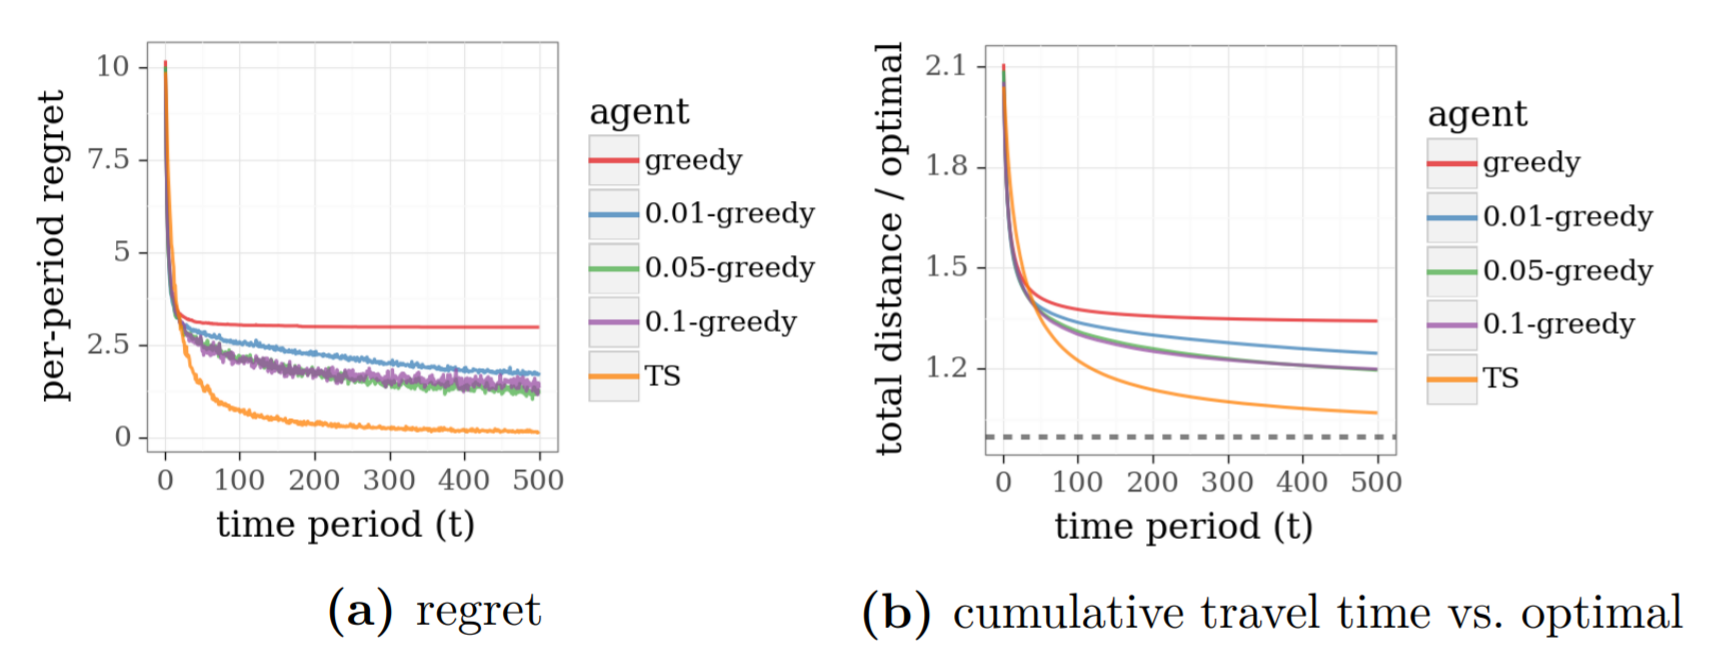
\includegraphics[keepaspectratio,
                     width=.9\paperwidth]{shortest_path_problem.png}
  \end{center}
\end{frame}


\begin{frame}
  \frametitle{Upper Confidence Bound}

  \begin{itemize}
    \item на основе исторических данных оценить распределение параметров модели $\Theta$, $P(\Theta|X)$
    \item выбираем действие $$ x_k = \arg\max_{x_k} (\mu_k^t + c \cdot u_k^t), \ \hat \Theta = E \Theta$$
    \item повторяем
  \end{itemize}

   $u_k^t$ характеризует нашу неуверенность в действии $x_k$ и не обязательно выражается через апостериорное распределение

  Например: $$ u_k^t = \sqrt{\frac{\log(t)}{|T_k|}}$$
\end{frame}


\begin{frame}
  \frametitle{Расширения и эвристики для семплирования Томпсона}

  {\bf Возможные проблемы}

  \begin{itemize}
    \item бизнес-ограничения
    \item контекст
    \item нестационарность
    \item многопоточность (например, много пользователей)
    \item подсчет апостериорного распределения
  \end{itemize}

\end{frame}


\begin{frame}
  \frametitle{Контекст}

  Пусть $y^t_i \sim q(y|x^t_i, z^t, \Theta)$

  В таком случае можно:
  \begin{itemize}
    \item $X = \{(x_i, z_j)\}$
    \item контекстуальные бандиты (LinUCB) — идея метода в том, что награда теперь зависит от контекста $z^t$, в качестве которого может выступать, например, вектор пользователя
  \end{itemize}

  \vspace{1cm}
  \noindent\rule{8cm}{0.4pt}

  {\small
  {\it Kuan-Hao Huang and Hsuan-Tien Lin.} Linear Upper Confidence Bound Algorithm for Contextual Bandit Problem with Piled Rewards
  \href{https://www.csie.ntu.edu.tw/~htlin/paper/doc/pakdd16piled.pdf}{https://www.csie.ntu.edu.tw/~htlin/paper/doc/pakdd16piled.pdf}}
\end{frame}


\begin{frame}
  \frametitle{Нестационарность}

  Пусть $y^t_i \sim q_t(y|x^t_i, \Theta)$

  В таком случае можно:
  \begin{itemize}
    \item аппроксимировать апостериорную вероятность по последней истории
    \item добавляем неуверенность
  \end{itemize}
  $$P_t(\Theta|Y_t) = \frac{q(y^t|x^t, \Theta) P^{1-\gamma}_{t-1}(\Theta|Y_{t-1}) \overline{P}^\gamma(\Theta)}{q(y^t|x^t)}$$

  к примеру в задаче про бандитов Бернулли
  $$(\alpha_k, \beta_k) \leftarrow
  \begin{cases}
  ((1-\gamma)\alpha_k + \gamma\overline{\alpha}, (1-\gamma)\beta_k + \gamma\overline{\beta}), \quad x_t \neq k \\
  ((1-\gamma)\alpha_k + \gamma\overline{\alpha} + r_t, (1-\gamma)\beta_k + \gamma\overline{\beta} + 1 - r_t), \quad x_t = k
  \end{cases}$$
\end{frame}


\begin{frame}
  \begin{center}
    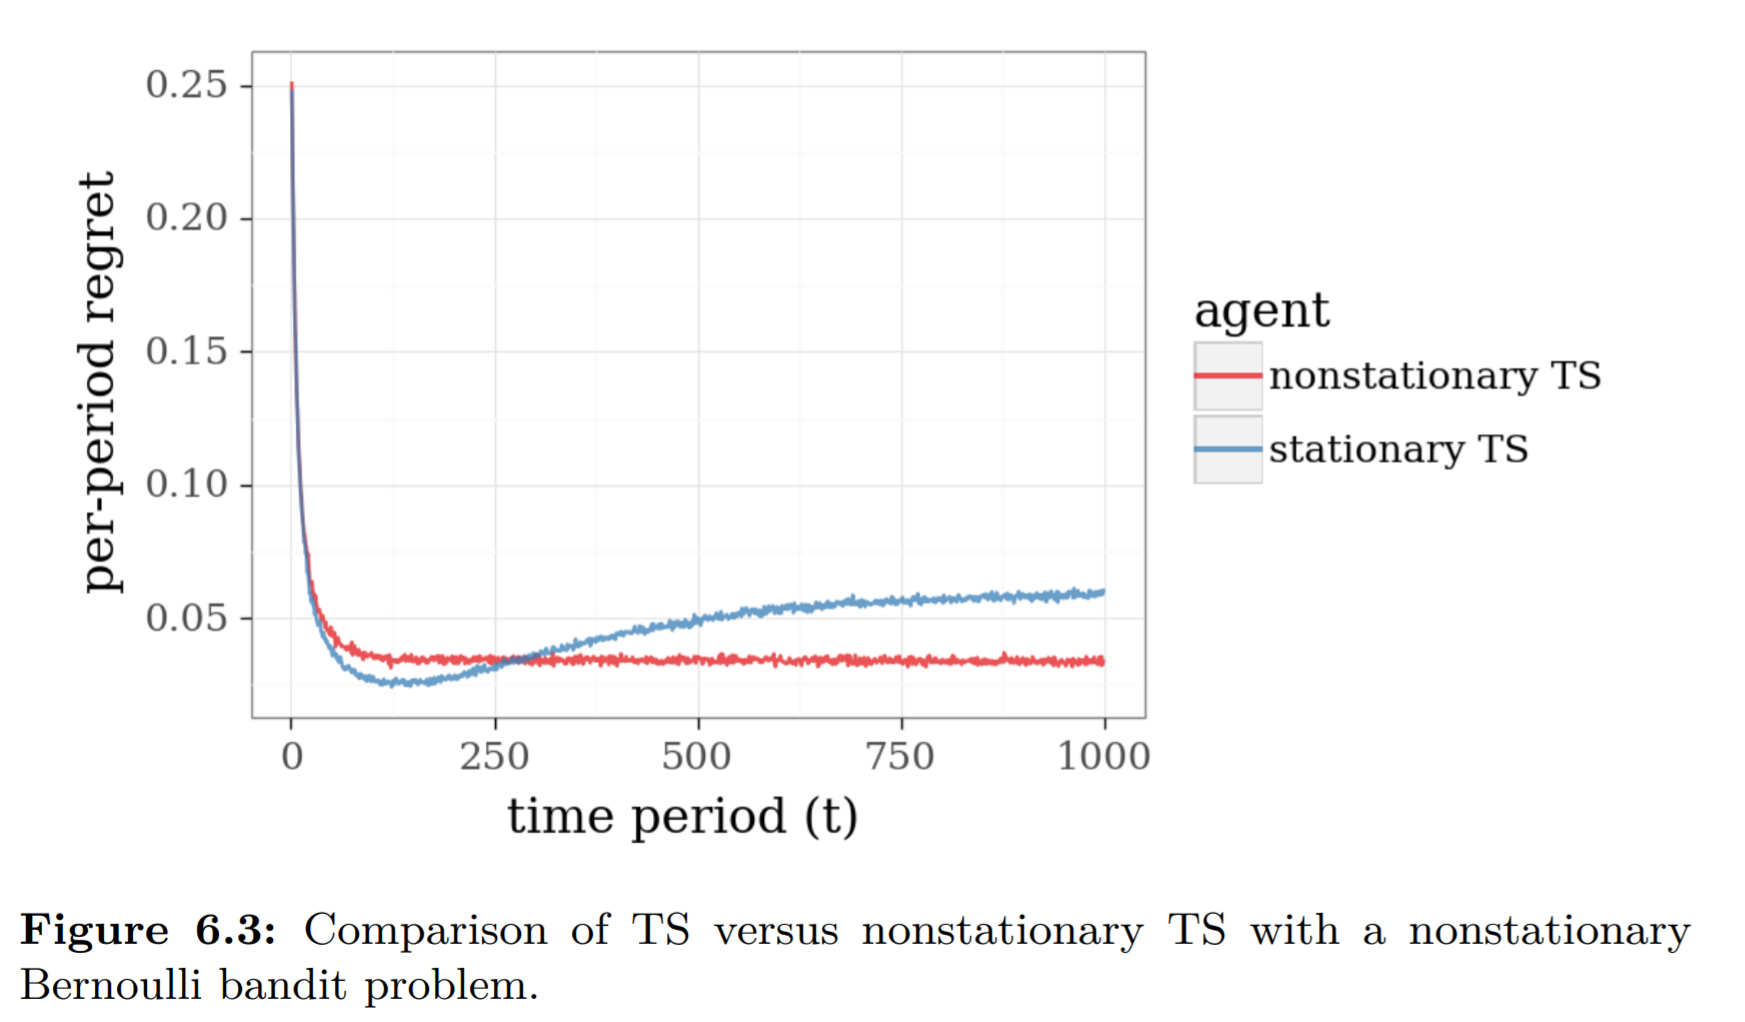
\includegraphics[keepaspectratio,
                     width=.9\paperwidth]{nonstationary_TS.png}
  \end{center}
\end{frame}


\begin{frame}
  \frametitle{Многопоточность}

  \begin{center}
    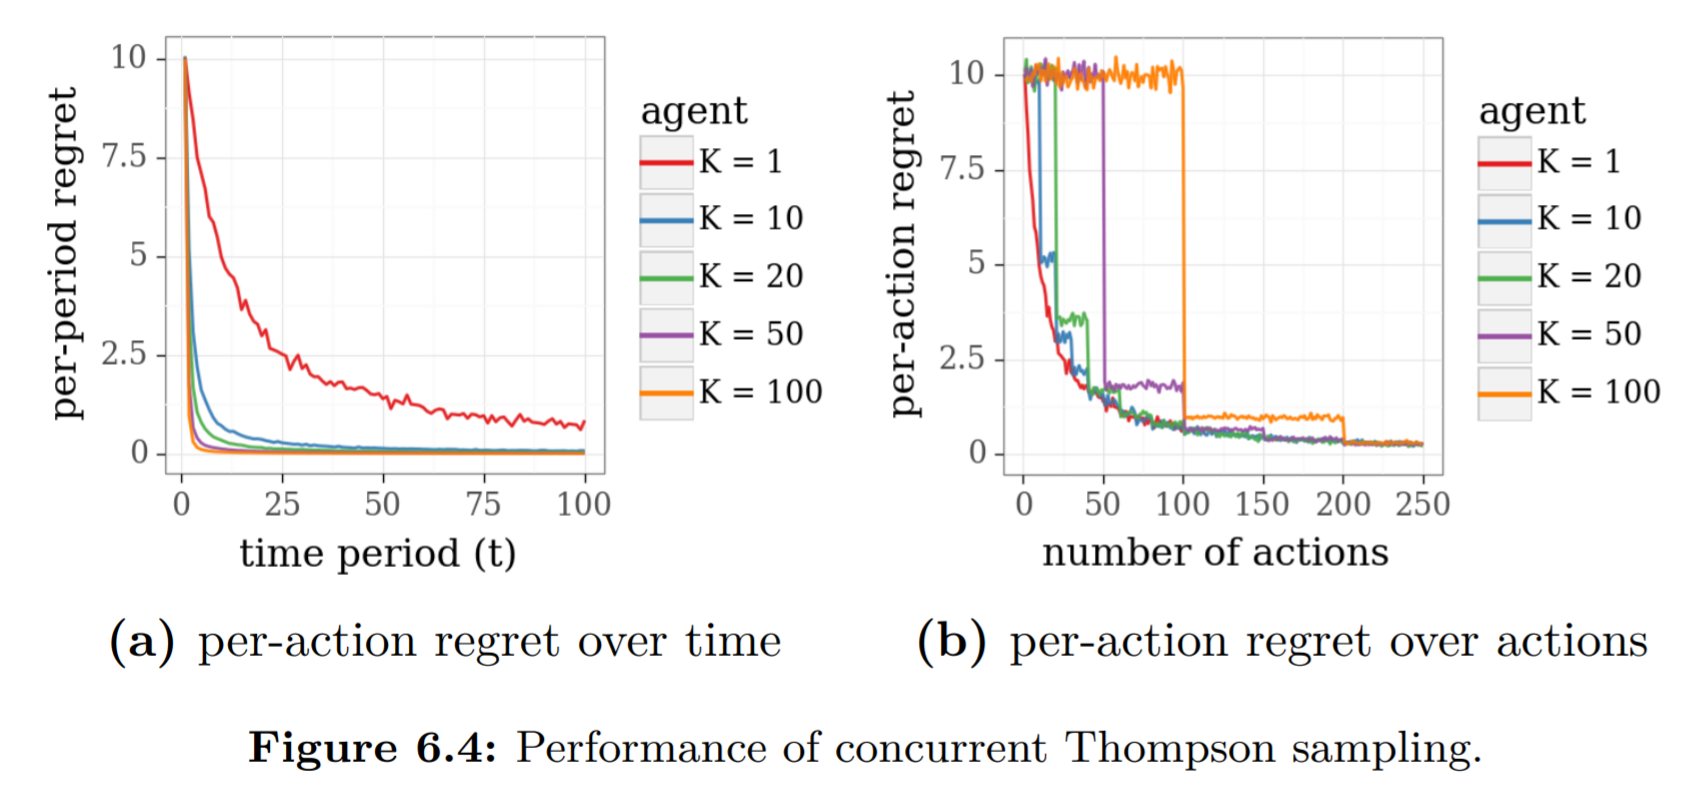
\includegraphics[keepaspectratio,
                     width=.9\paperwidth]{concurrent.png}
  \end{center}
\end{frame}


\begin{frame}
  \frametitle{Снова аппроксимации апостериорного распределения}

  \begin{itemize}
    \item сэмплирование Гиббса
    \item Langevin Monte Carlo
    \item приближенный вариационный вывод (аппроксимация Лапласа)
    \item bootstrap
  \end{itemize}

  \begin{center}
    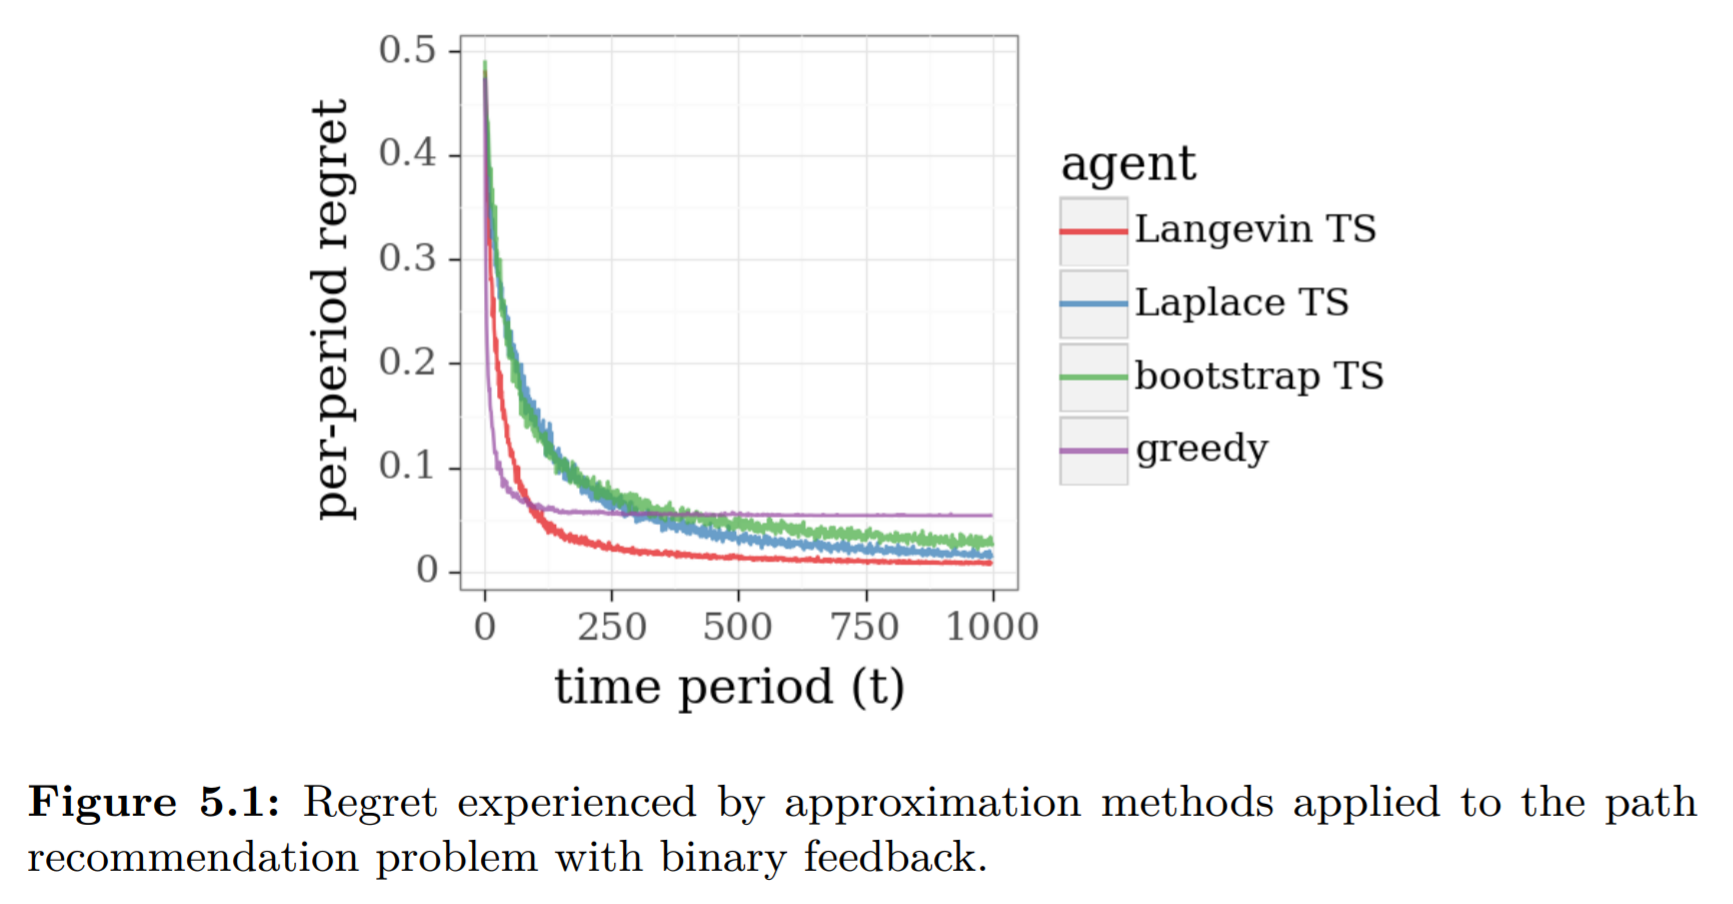
\includegraphics[keepaspectratio,
                     width=.7\paperwidth]{tompson_sampling.png}
  \end{center}
\end{frame}


\begin{frame}
  \frametitle{Области применения}

  \begin{itemize}
    \item revenue management
    \item оптимизация сайтов
    \item интернет-реклама
    \item рекомендательные системы
    \item продвижение контента
    \item обучение нейронных сетей
  \end{itemize}
\end{frame}


\begin{frame}[t]
  \frametitle{Резюме}

  \begin{itemize}
    \item многорукие бандиты — частный случай обучения с подкреплением
    \item $\varepsilon$-жадный алгоритм и сэмплирование Томпсона
    \item UCB — upper confidence bound
    \item способы аппроксимации апостериорного распределения
  \end{itemize}
  \vspace{1cm}
  \pause
  Что ещё можно посмотреть?

  \begin{itemize}
    \item Видео \href{https://www.youtube.com/watch?v=SfSqLn0j10g}{«A short introduction to multi-armed bandits»}
    \item Книга \href{https://arxiv.org/abs/1904.07272}{«Introduction to Multi-Armed Bandits»}, Aleksandrs Slivkins
    \item Книга \href{https://arxiv.org/pdf/1707.02038.pdf}{«A Tutorial on Thompson Sampling»}
  \end{itemize}
\end{frame}

\end{document}
